\documentclass[fleqn,10pt]{SelfArx} 

\usepackage[utf-8]{babel} 
%----------------------------------------------------------------------------------------
%	COLUMNS
%----------------------------------------------------------------------------------------

\setlength{\columnsep}{0.55cm} 
\setlength{\fboxrule}{0.75pt} 
\usepackage[english]{babel} % Specify a different language here - english by default
\usepackage{lipsum} % Required to insert dummy text. To be removed otherwise
\usepackage{amsmath}
\graphicspath{ {./Imagenes/} }
%----------------------------------------------------------------------------------------
%	COLORS
%----------------------------------------------------------------------------------------

\definecolor{color1}{RGB}{0,0,90} % Color of the article title and sections
\definecolor{color2}{RGB}{230, 231, 231} % Color of the boxes behind the abstract and headings

%----------------------------------------------------------------------------------------
%	HYPERLINKS
%----------------------------------------------------------------------------------------

\usepackage{hyperref} % Required for hyperlinks

\hypersetup{
	hidelinks,
	colorlinks,
	breaklinks=true,
	urlcolor=color2,
	citecolor=color1,
	linkcolor=color1,
	bookmarksopen=false,
	pdftitle={Title},
	pdfauthor={Author},
}

%----------------------------------------------------------------------------------------
%	ARTICLE INFORMATION
%----------------------------------------------------------------------------------------

\JournalInfo{Método de Muller, 2022} % Journal information

\PaperTitle{Método de Muller} % Article title

\Authors{Juan Páez\textsuperscript{1}, Santiago Zuñiga\textsuperscript{2}} % Authors
\affiliation{\textsuperscript{1}\textit{Facultad de ingeniería, Pontificia Universidad Javeriana}} % Author affiliation
\affiliation{\textsuperscript{2}\textit{Facultad de ingeniería, Pontificia Universidad Javeriana}} % Author affiliation
\affiliation{\textbf{Autor correspondiente}: jd.paez@javeriana.edu.co} % Corresponding author

\Keywords{Muller --- Solution --- Complex Roots --- One Variable --- Error} % Keywords - if you don't want any simply remove all the text between the curly brackets
\newcommand{\keywordname}{Keywords} % Defines the keywords heading name

%----------------------------------------------------------------------------------------
%	ABSTRACT
%----------------------------------------------------------------------------------------

\Abstract{In this paper we will explain the Muller method used 
to solve equations in one variable with complex roots, we will also 
present an application problem with the computational solution and 
the respective error analysis.}

%----------------------------------------------------------------------------------------

\begin{document}

\maketitle % Output the title and abstract box

\thispagestyle{empty} % Removes page numbering from the first page

%----------------------------------------------------------------------------------------
%	ARTICLE CONTENTS
%----------------------------------------------------------------------------------------

\section*{Introducción} % The \section*{} command stops section numbering

\addcontentsline{toc}{section}{Introduction} % Adds this section to the table of contents
A la hora de solucionar ecuaciones no lineales en una variable, 
es decir encontrar o aproximar sus raíces, se pueden utilizar 
distintos métodos, como el despeje directo, Newton, posición falsa, 
entre otros. Sin embargo, se presenta un problema cuando las funciones que 
queramos evaluar tengan raíces complejas, ya que los métodos mencionados
no son los indicados para este tipo planteamientos. 
Es por eso que el matemático estadounidense, David Eugene \textbf{Muller}, 
propuso un método para poder obtener un aproximación de este tipo de 
funciones el cual será explicado y desarrollado a lo largo de este documento.


%------------------------------------------------

\section{Definición}

El método de Muller, esta muy relacionado con el método de la secante, 
teniendo en cuenta que este consiste en tener una aproximación de la 
raíz a partir de dos puntos en la función $f(x)$. 

\begin{figure}[ht]\centering
	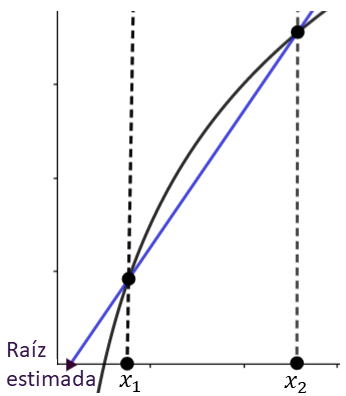
\includegraphics[scale=0.5]{GrafSecante.png}\\\ 
	\caption{Método de la secante}
	\label{fig:secante}
\end{figure}
En el caso de 
Muller consiste en tener 3 puntos sobre la gráfica de la función, 
siendo estos una composición cuadrática, la cual da una aproximación de la solución o raíz de $f(x)$.
\begin{figure}[ht]\centering
	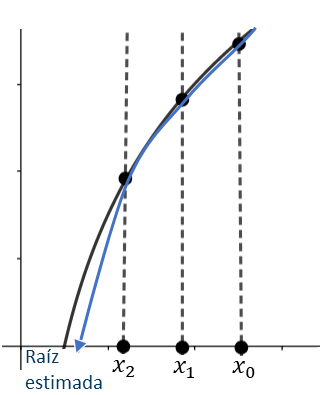
\includegraphics[scale=0.5]{GrafMuller.png}\\\
	
	\caption{Método de Muller}
	\label{fig:muller}
\end{figure}

\subsection{Definición matemática}

Teniendo en cuenta la forma general de la ecuación cuadrática y la aproximación de la raíz,
el metodo comienza planteando el siguiente polinomio cuadrático:
\begin{equation} \label{eq:formaGeneral}
	g(x)=a(x-x_{2})^2+b(x-x_{2})+c
\end{equation}
Queremos que la función $g(x)$, representada de color azul, pase por los puntos presentados en la figura \ref*{fig:muller},
 es decir $[x_{0},f(x_{0})]$ , $[x_{1},f(x_{1})]$ y $[x_{2},f(x_{2})]$, por lo tanto sustituyendo en la ecuación (\ref*{eq:formaGeneral}),
 nos da las respectivas imagenes de las funciones en $g(x_{k})$.

\begin{equation} \label{eq:g0}
\begin{aligned}
	g(x_{0})=a(x_{0}-x_{2})^2+b(x_{0}-x_{2})+c
\end{aligned}
\end{equation}
\begin{equation} \label{eq:g1}
\begin{aligned}
	g(x_{1})=a(x_{1}-x_{2})^2+b(x_{1}-x_{2})+c
\end{aligned}
\end{equation}
\begin{equation} \label{eq:g2}
\begin{aligned}
	g(x_{2})=a(x_{2}-x_{2})^2+b(x_{2}-x_{2})+c
\end{aligned}
\end{equation}
Al haber tres ecuaciones, podemos hallar los valores de los tres coeficientes $a$,$b$ y $c$.
Empezando por el valor de $c$, que utilizando la ecuación (\ref*{eq:g2}) sería:
\begin{equation} \label{eq:g2S}
	\begin{aligned}
	g(x_{2})=a(0)^2+b(0)+c\\
	g(x_{2})=c
\end{aligned}
\end{equation}

%\section{Results and Discussion}

\end{document}